\documentclass[border=4pt]{standalone}
\usepackage{amsmath}
\usepackage{tikz}
\usetikzlibrary{shapes.geometric,arrows.meta,positioning,fit}
\begin{document}
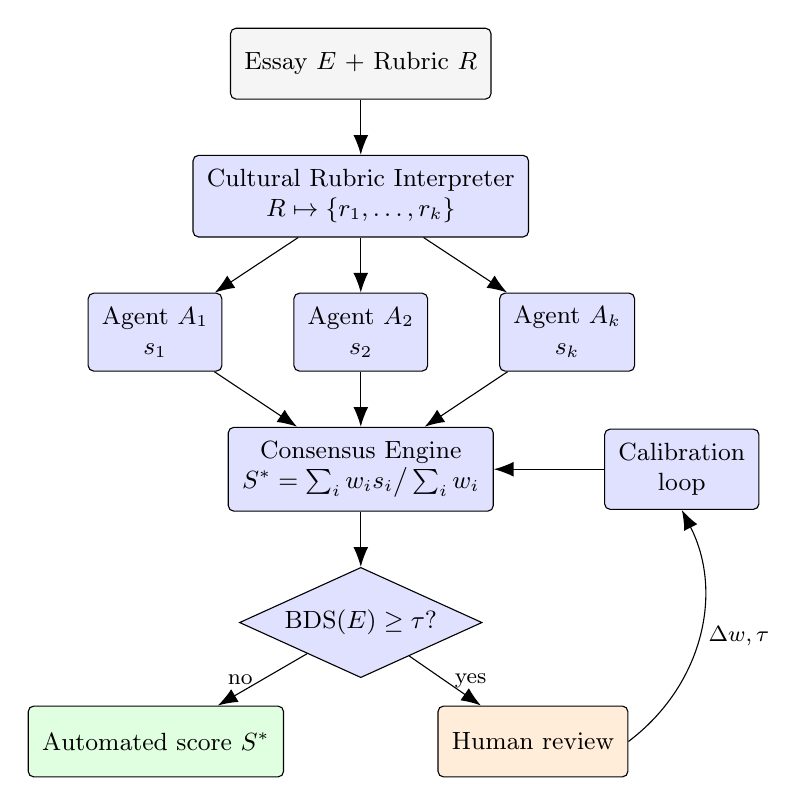
\begin{tikzpicture}[
  node distance=7mm and 9mm,
  box/.style={rectangle, rounded corners=2pt, draw, align=center,
              minimum height=9mm, inner sep=5pt, font=\small},
  comp/.style={box, fill=blue!12},
  agent/.style={box, fill=blue!12},
  io/.style={box, fill=gray!8},
  outcome/.style={box, fill=green!12},
  humanbox/.style={box, fill=orange!15},
  decide/.style={diamond, aspect=2.2, draw, align=center, font=\small,
                 inner sep=2pt, fill=blue!12},
  arr/.style={-{Latex[length=2.5mm]}}]
  \node[io] (input) {Essay $E$ + Rubric $R$};
  \node[comp, below=of input] (cri) {Cultural Rubric Interpreter\\
        $R \mapsto \{r_1, \dots, r_k\}$};
  \node[agent, below=of cri] (a2) {Agent $A_2$\\$s_2$};
  \node[agent, left=of a2] (a1) {Agent $A_1$\\$s_1$};
  \node[agent, right=of a2] (ak) {Agent $A_k$\\$s_k$};
  \node[comp, below=of a2] (cons) {Consensus Engine\\
        $S^{*} = \sum_i w_i s_i \big/ \sum_i w_i$};
  \node[decide, below=of cons] (bds) {$\mathrm{BDS}(E) \geq \tau$?};
  \node[outcome, below left=7mm and 2mm of bds] (score) {Automated score $S^{*}$};
  \node[humanbox, below right=7mm and 2mm of bds] (human) {Human review};
  \node[comp, right=14mm of cons, font=\small] (cal) {Calibration\\loop};
  \draw[arr] (input) -- (cri);
  \draw[arr] (cri) -- (a1);
  \draw[arr] (cri) -- (a2);
  \draw[arr] (cri) -- (ak);
  \draw[arr] (a1) -- (cons);
  \draw[arr] (a2) -- (cons);
  \draw[arr] (ak) -- (cons);
  \draw[arr] (cons) -- (bds);
  \draw[arr] (bds) -- node[left, font=\footnotesize]{no} (score);
  \draw[arr] (bds) -- node[right, font=\footnotesize]{yes} (human);
  \draw[arr] (human.east) to[bend right=40] node[right, font=\footnotesize]{$\Delta w, \tau$} (cal.south);
  \draw[arr] (cal) -- (cons);
\end{tikzpicture}
\end{document}
